\documentclass[11pt,letterpaper]{article}
\usepackage[lmargin=1in,rmargin=1in,tmargin=1in,bmargin=1in]{geometry}
\usepackage{../style/quiz}
\setbool{hideans}{true} % Student: True; Instructor: False

% -------------------
% Content
% -------------------
\begin{document}
\quiz{9}

% Problem 1
\problem Determine whether the table below could represent an exponential function, $f(x)$. Be sure to justify why or why not. \par
	\begin{table}[!ht]
	\centering
	\begin{tabular}{|c||cccc|} \hline
	$x$ & $1$ & $2$ & $3$ & $4$ \\ \hline
	$f(x)$ & $3$ & $4.5$ & $6.75$ & $10.125$ \\ \hline
	\end{tabular}
	\end{table} \par

\ans{This can represent an exponential function. An exponential function is a function which has a constant ratio between terms. Observe that $\frac{4.5}{3}= 1.5$, $\frac{6.75}{4.5}= 1.5$, and $\frac{10.125}{6.75}= 1.5$. That is, each subsequent term is obtained by taking the previous value and multiplying by $1.5$. In fact, $f(x)= 2(1.5)^x$.} \pvspace{1.5cm} \vfill



% Problem 2
\problem Consider the function $f(x)= 7(1.38)^x$.
	\begin{enumerate}[(a)]
	\item Determine $A$ and $b$ for this exponential function. \vfill
	\ans{An exponential function has the form $Ab^x$. Observe that here $A= 7$ and $b= 1.38$.} \vfill
	
	\item What is the $y$-intercept for $f(x)$? \vfill
	\ans{The $y$-intercept for an exponential function is the $A$-value. From (a), we know that $A= 7$. Therefore, the $y$-intercept is $7$. Alternatively, the $y$-intercept is the value when $x= 0$. We have $f(0)= 7(1.38)^0= 7(1)= 7$.} \vfill
	
	\item Determine the growth or shrink rate for $f(x)$. \vfill
	\ans{If $f(x)= A(1 + g)^x$, where $g > 0$, then $f(x)$ is growing exponentially and the growth rate is $g$---written as a percentage. If $f(x)= A(1 - g)^x$, where $g > 0$, then $f(x)$ is shrinking exponentially and the shrink rate is $g$. We know from (a) that $b= 1.38$. We write $b= 1.38= 1 + 0.38$. Therefore, $f(x)$ is growing exponentially with growth rate 38\%.} \vfill
	\end{enumerate} \vfill



% Problem 3
\problem Let $y= 2^{2 - x}$. Determine whether $y$ is exponentially growing or decaying. Be sure to justify your answer. Sketch $y$ below. \par\vspace{0.1cm}
\begin{minipage}[t]{0.48\textwidth}
	\fbox{
	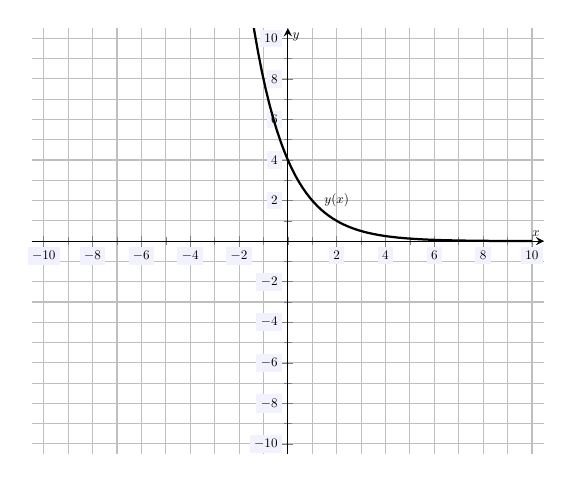
\begin{tikzpicture}[scale=0.95,every node/.style={scale=0.5}]
	\begin{axis}[
	grid=both,
	axis lines=middle,
	ticklabel style={fill=blue!5!white},
	xmin= -10.5, xmax=10.5,
	ymin= -10.5, ymax=10.5,
	xtick={-10,-8,...,10},
	ytick={-10,-8,...,10},
	minor tick = {-10,-9,...,10},
	xlabel=\(x\),ylabel=\(y\),
	]
	\remove{\node at (2,2) {$y(x)$};}
	\remove{\addplot[line width= 0.03cm,samples=100,domain= -5:10] ({x},{2^(2 - x)});}

	\end{axis}
	\end{tikzpicture}
	}
\end{minipage}\begin{minipage}[b]{0.48\textwidth}
\wans{We write\dots
	\[
	y= 2^{2 - x}= 2^2 2^{-x}= 4(2^{-x})= 4(2^{-1})^x= 4 \left( \dfrac{1}{2} \right)^x
	\]
This is an exponential function $Ab^x$ with $A= 4$ and $b= \frac{1}{2}$. Because $A= 4$, the $y$-intercept is $4$. Because $b= \frac{1}{2}$ and $0 < b < 1$, we know that the function is shrinking exponentially. We then sketch this function on the left. \vspace{0.5cm} \phantom{x}}
\end{minipage} \vfill

\end{document}